%
% SecMeas: Experimental results
%

In this section, we presents our experimental results obtained so far. While the ultimate goal is to implement Mobile Vital Radio on cell phone, at the current phase of the project we are transmitting signal using laptop's speaker and receiving signal using cell phone. The FFT is performed using MATLAB by uploading the audio files of transmitted and received signals to the laptop. In order to correctly start the peak search, we need to first run a cross-correlation between the transmission and reception since we are currently employing two different devices. Based on the correlation result, we are able to identify the starting point of our FFT.

%
\begin{figure}[!htbp]
	\centering
	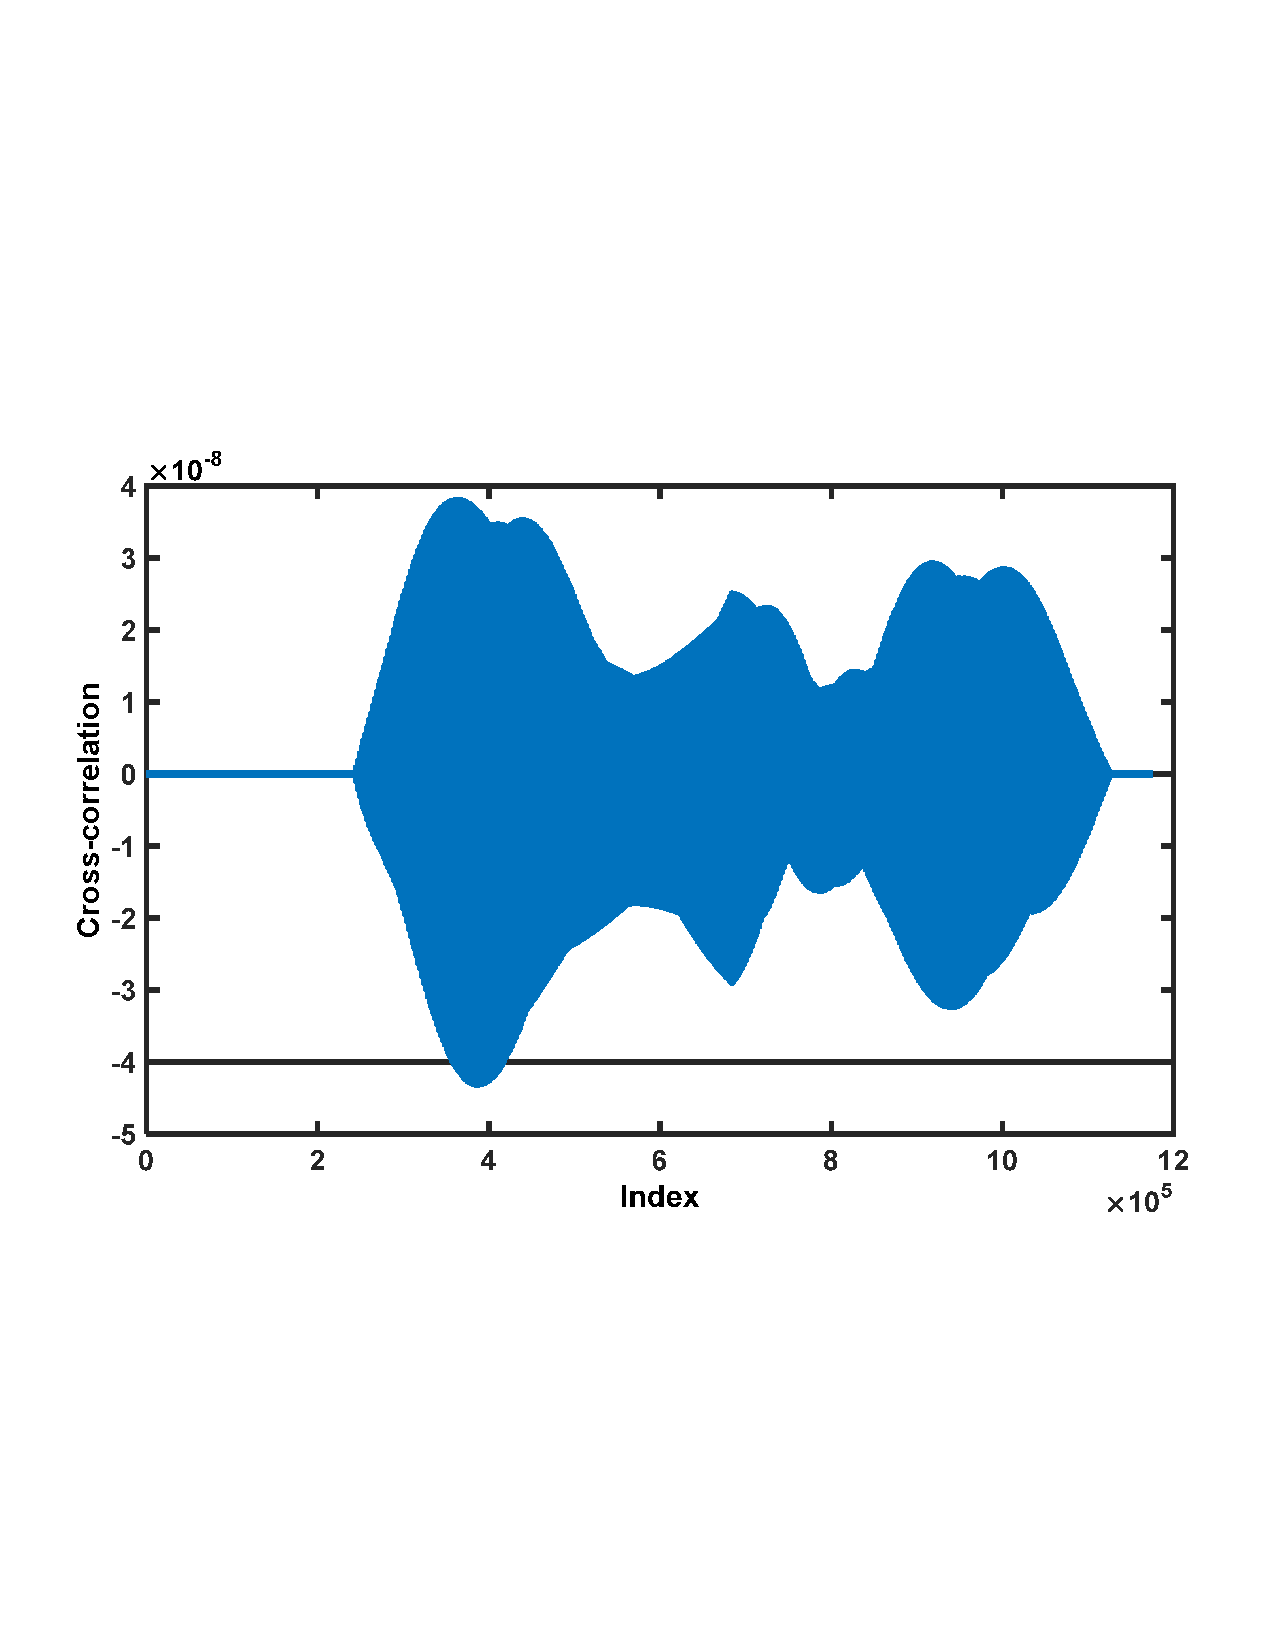
\includegraphics[width=0.9\columnwidth]{Fig02_corr}
	\captionsetup{justification=raggedright, singlelinecheck=false}
	\caption{Cross-correlation between transmitted and received signal of FMCW transmission.}
	\label{fig:corr}
\end{figure}
%

As shown in Fig.~\ref{fig:corr}, the cross-correlation of the two audio files does not show a peak indicating the index shift required corresponding to the distance offset between our position of speaker and microphone. Instead, the obtained cross-correlation actually shows amplitude-modulated waveform, which we believe is caused due to the sampling frequency offset between the two devices. In order to resolve such discrepancy between hardwares, we decide to first design an android application that is able to access both the microphone and speak of the cell phone so that the testing setup could be conducted using cell phone only. 

Next, we tested the possibility to identify static and dynamic object (assuming only one at presence) in the environment. For this experiment, we run the peak search and choose the first five peaks identified in the spectrum. As shown in Fig.~\ref{fig:path}, we are able to correctly identify the movement of the object (data 5 in the plotted figure). Small fluctuations are observed due to the fact that we have to manually press the recording and move away from the cell phone to prevent further disturbance. However, such action may still result in unnecessary noise in the process. We hope to address the issue with the android application.

%
\begin{figure}[!htbp]
	\centering
	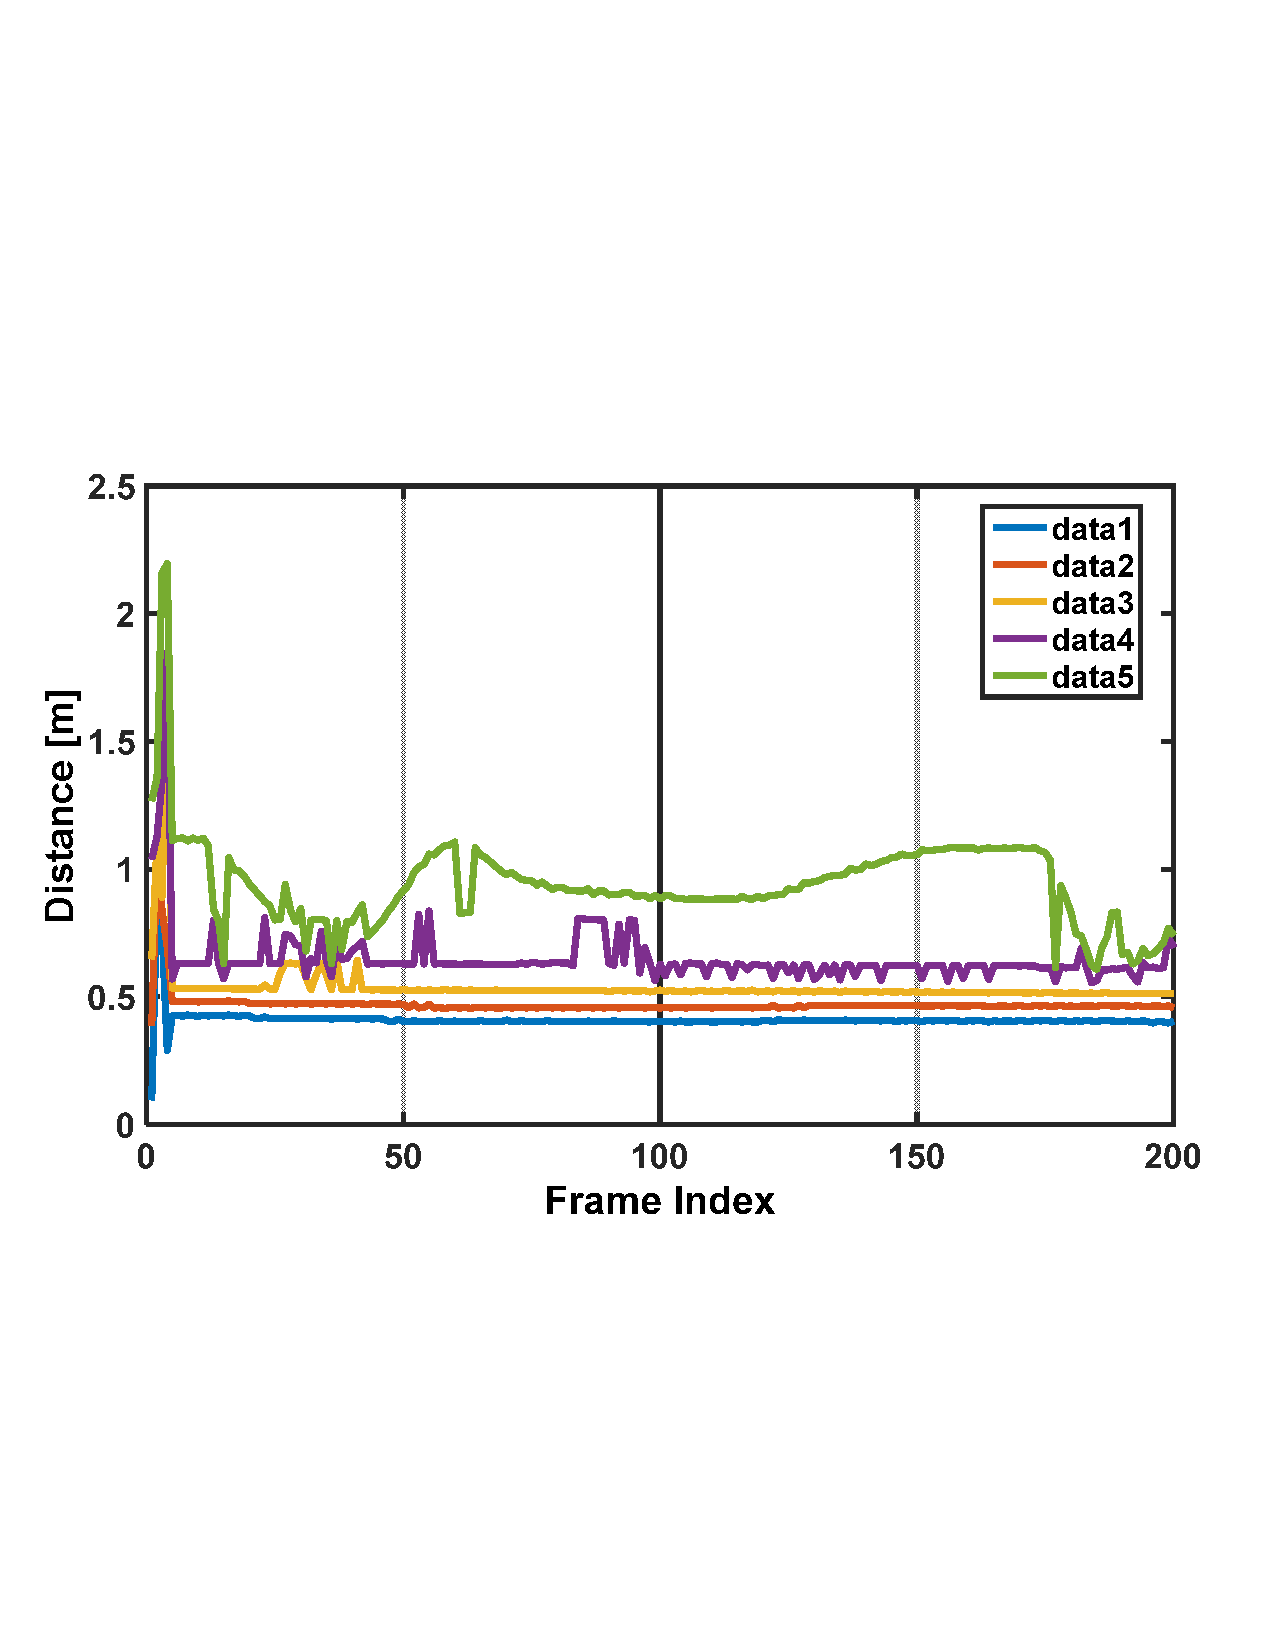
\includegraphics[width=0.9\columnwidth]{Fig03_path}
	\captionsetup{justification=raggedright, singlelinecheck=false}
	\caption{Path profile demonstrates that we are able to identify static and dynamic object in the environment.}
	\label{fig:path}
\end{figure}
%



